% Chapter Template

\chapter{SVM} % Main chapter title

\label{Chapitre 4.1} % Change X to a consecutive number; for referencing this chapter elsewhere, use \ref{ChapterX}

\lhead{ \emph{}} % Change X to a consecutive number; this is for the header on each page - perhaps a shortened title

%----------------------------------------------------------------------------------------
%	SECTION 1
%----------------------------------------------------------------------------------------
\section{Entrainement de la SVM}

Nous lisons les données et séparons le set de données avec les méthodes suivantes:
\begin{lstlisting}[frame=single,style=Python]
X, y = load_data(data_path)
        X_train, X_test, y_train, y_test = cross_validation.train_test_split(X, y, test_size=0.4, random_state=0)
\end{lstlisting}

Nous n'avons pas vérifié le fonctionnement exacte de la méthode cross_validation.train_test_split. Nous lui faisons confiance pour qu'elle partage les données en set d'entrainnement et de test d'une bonne façon.

La matrice de confusion après la cross validation est la suivante:
\begin{center} 
\hspace{12.45cm}
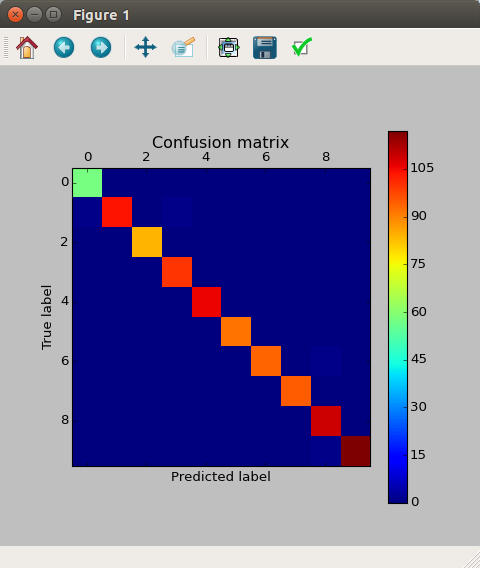
\includegraphics[width=10cm]{ConfusionMatrixSvmTrainning.png}
\end{center}

Les résultats sont bons puisque tous les chiffres sont reconnus à au moins 60\%.

